\documentclass[mathserif]{beamer}
\usetheme{Berlin} %sidebar
\usecolortheme{dolphin}
\newcommand{\bi}{\begin{itemize}\item}
\newcommand{\ei}{\end{itemize}}

\newcommand{\inner}[2]{\big<\vec{#1}\cdot\vec{#2}\big>}
%\include{../beamer_presentation}


\title[Supervised Learning Linear Priority Dispatch Rules for Job-Shop Scheduling \qquad\; Learning and Intelligent OptimizatioN (LION 5)]{Supervised Learning Linear Priority Dispatch Rules for Job-Shop Scheduling}
\author{Helga Ingimundardottir \& Thomas Philip Runarsson}
\date{20th of January, 2011} % beskidt .. men det virker
\institute{School of Engineering and Natural Sciences, University of Iceland}


% \beamertemplatenavigationsymbolsempty % fjerner pdf-indhold


%\AtBeginSection[]{\begin{frame}<beamer>   \frametitle{Overview}    \tableofcontents[currentsection]  \end{frame} }


%%%%%%%%%%%%%%%%%%%%%%%%%%%%%%%%%%%%%%
\begin{document}
%%%%%%%%%%%%%%%%%%%%%%%%%%%%%%%%%%%%%%
\frame{\titlepage}

\frame{\frametitle{Overview}
\begin{enumerate}
 \item Introduction
  \item Job Shop Scheduling Problem
\bi Mathematical formulation
\item Dispatching rules
\item Features for JSSP
\item Data generation
\item Logistic regression
\ei
\item Experimental Study
\bi Technical setup
\item Main conclusions
\ei
\item Future Work
\end{enumerate}

}

%\section{Abstract}
%\frame{\frametitle{Abstract}
%\bi Introduction to a framework in which dispatching rules for \emph{job-shop scheduling problems} (JSSP) are discovered with supervised learning by analyzing characteristics of optimal solutions. 
%  \item Ordinal regression implemented to identify good choices from bad at each time step.
%  \item Data-driven method.
%  \item Robust towards scalability and different data distributions. 
%  \item Dispatching rules from this new framework outperform the most common single priority-based dispatching rules w.r.t. minimum makespan. 
%  \item Experiments on simulated data. 
%\ei
%}

\section{Introduction}
\frame{\frametitle{Goal}
\bi General goal is how to search for \emph{good} solutions for an arbitrary problem domain. 
  \item To automate the design of optimization algorithms.
  \item In this work we learn new dispatching rules for JSSP
  \item Using randomly sampled problem instances and their corresponding optimal solutions.
\ei
}
\frame{\frametitle{Previous work}
Methods previously proposed for solving JSSP:
\bi Genetic programming, e.g. Tay \& Ho (2008)
  \item Reinforcement learning, e.g. Zhang \& Dietterich (1995)
  \item Regression trees, e.g. Li \& Olafsson (2005)
\ei 
}
\section{Job Shop Scheduling}
\subsection{Mathematical formulation}
\frame{\frametitle{Job Shop Scheduling}
\bi Job shop scheduling consists of a set of $n$ jobs that must be scheduled on a set of $m$ machines. 
\item Each job has an indivisible operation time on machine% $a$, $p(j,a)$
%\item Starting time of job $j$ on machine $a$ is denoted $x_s(a,j)$ and its completion time is denoted $x_f$ and
%$$x_f(a,j)=x_s(a,j)+p(j,a) $$
\item The time in which machine is idle is called slack time, 
%$$s(a,j)=x_s(a,j)-x_f(a,j-1). $$
%\ei
%}
%\frame{\frametitle{Job Shop Scheduling}
\item Each job must follow a predefined machine order%: 
%$$   x_s( \sigma(j,a),j) \geq x_f(\sigma(j,a-1),j) \quad j\in\{1,..,n\},\; a\in\{2,..,m\}$$
\item Each machine can handle at most one job at a time%:
%$$   x_s(a,i) \geq x_f(a,j) \quad\textrm{or}\quad x_s(a,j) \geq x_f(a,i)  $$
\item Optimal schedule is the one where the time to complete all jobs is minimal (minimum makespan).
%$$  z = \max\{x_f(j,m)\;|\;j=1,..,n\}.$$
\ei
}
\subsection{Dispatching rules}
\frame{\frametitle{Example of Job Shop Scheduling} 
\begin{figure}[b!]
\centering
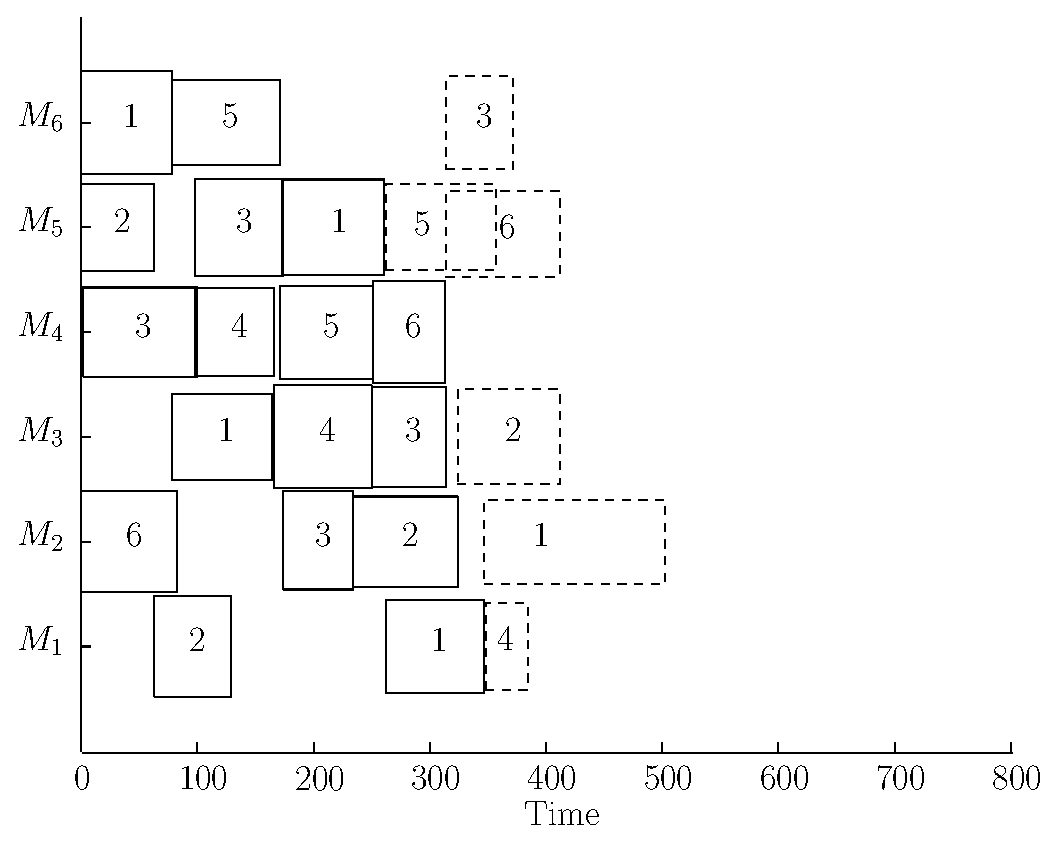
\includegraphics[width=0.50\columnwidth]{figs/dispatch_features.eps}
\caption{A schedule being built, the dashed boxes represent six different possible jobs that could be scheduled next using a dispatch rule.}
\end{figure}
}
\frame{\frametitle{Dispatching rules for solving JSSP}
\bi Dispatching rules are of a construction heuristics, where one starts with an empty schedule and adds on one job at a time. 

\item When a machine is free the dispatching rule inspects the waiting jobs and selects the job with the highest priority. 

\item Most effective single priority based dispatch rules:
  \bi Most work remaining (MWRM)
    \item Least work remaining (LWRM)
    \item Shortest processing time (SPT)
    \item Largest processing time (LPT)
  \ei
\ei
}
\subsection{Feature for JSSP}
\frame{\frametitle{Feature selection}
\begin{table}[h!]
 {\footnotesize
 \begin{center}
  \begin{tabular}{|c|p{5cm}|}
   \hline\hline
  feature &  description \\ \hline
  $\phi(1)$ & processing time for job on machine\\
  $\phi(2)$ & work remaining \\
  $\phi(3)$ & start-time \\
  $\phi(4)$ & end-time \\
  $\phi(5)$ & when machine is next free \\
  $\phi(6)$ & current makespan \\
  $\phi(7)$ & slack time for this particular machine \\
  $\phi(8)$ & slack time for all machines \\
  $\phi(9)$ & slack time weighted w.r.t. number of operations already assigned \\
   \hline\hline
  \end{tabular}
 \end{center}}
 \caption{Features for JSSP}
\end{table}
}
\subsection{Data generation}
%\frame{\frametitle{Data generation}
%\bi Data distributions
% \bi $U(1,100)$
%  \item $U(50,100)$
% \ei
% \item Size of data sets:
% \bi Training set: 200  
%  \item Validation set: 100
%  \item Test set: 200
% \ei
%\ei
%}
\frame{\frametitle{Generating training data}
\bi Determine the order (sequence) of jobs assigned, at the first available time slot (to the left)
  \item When job is assigned, new state occurs and features are updated
  \item At each time step, a good/bad ordinal data pair is only created if final makespan is different.
  \bi At least one or more optimal solution for each JSSP 
    \item Sequence representation is not uniquely determined.
  \ei
\ei
}
\frame{\frametitle{Preference learning}
\bi The preference learning problem is specified by a set of point/rank pairs:
\bi Optimal decision: $\vec{z_o}=\vec{\phi}^{(o)}-\vec{\phi}^{(n)}$, ranked $+1$
\item Non-optimal decision: $\vec{z_n}=\vec{\phi}^{(n)}-\vec{\phi}^{(o)}$, ranked $-1$
\item In this study the training set is created from known optimal sequences of dispatch.
\ei
%\item Training set consists of the set:
%$$S = \left\{\left\{\vec{\phi}^{(o)}-\vec{\phi}^{(s)}_j,+1)\right\}_{i=1}^{\ell},%\left\{\vec{\phi}^{(s)}_j-\vec{\phi}^{(o)},-1)\right\}_{i=1}^{\ell}
%\;|\;\forall j\in J^{(k)}
%\right\}
%$$
%where $S\subset \Phi\times Y$ and $\Phi\subset \mathbb{R}^d$ is the training set of $d$ features, $Y=\{-1,+1\}$ is the outcome space, $\ell$ is the total number of dispatches and $j\in J^{(k)}$ are the possible suboptimal dispatches at dispatch $(k)$. 
\ei
}
\subsection{Logistic regression}
\frame{\frametitle{Logistic regression}
\bi Mapping of points to ranks: $ \{h(\cdot) : \Phi \mapsto Y\}$
\bi $\vec{\phi}_o \succ \vec{\phi}_s \quad \Leftrightarrow \quad h(\vec{\phi}_o) > h(\vec{\phi}_s)$ \ei
\item Logistical regression: obtain function $h^*$ that can for a given pair $(\vec{\phi}_i,y_i)$ and $(\vec{\phi}_j,y_j)$ distinguish between two different outcomes: $y_i > y_j$ and $y_j > y_i$. 
\item Problem of predicting the relative ordering of all possible pairs of examples
%\item The training set, composed of pairs, is then as follows: $$S' = \big\{(\vec{\phi}_k^{(1)}, \vec{\phi}_k^{(2)}),t_k=\text{sign}(y_k^{(1)} - y_k^{(2)})\big\}_{k=1}^{\ell'}$$ where $(y_k^{(1)} = r_i) \wedge (y_k^{(2)} = r_{i+1})$ (and vice versa) %$(y_k^{(1)} = r_{i+1}) \wedge (y_k^{(2)} = r_{i})$) resulting in $\ell'=2(\ell-1)$ possible adjacently ranked training pairs. 
%\item Rank difference is denoted by $t_k\in[-1,1]$.
\ei
% We deal only in the linear case for now...
%In order to generalize the technique to different point data types and model spaces an implicit kernel-defined feature space with corresponding feature mapping $\phi$ is applied. Consider the feature vector $\phi(\vec{\phi})=[\phi_1(\vec{\phi}),\ldots,\phi_m(\vec{\phi})]^T\in \reals^m$ where $m$ is the number of features. Then the surrogate considered may be defined by a linear function in the kernel-defined feature space: 
The surrogate considered may be defined by a linear function in the feature space:
$$
h(\vec{\phi}) = \sum_{i=1}^m w_i \vec{\phi} = \inner{w}{\phi}. %h(\vec{\phi}) = \sum_{i=1}^m w_i\phi_i(\vec{\phi}) = \inner{w}{\phi(\vec{\phi})}.
$$
}

\section{Experimental study}
\subsection{Technical setup}
\frame{\frametitle{Training size}
\begin{center}\begin{figure}[H] 
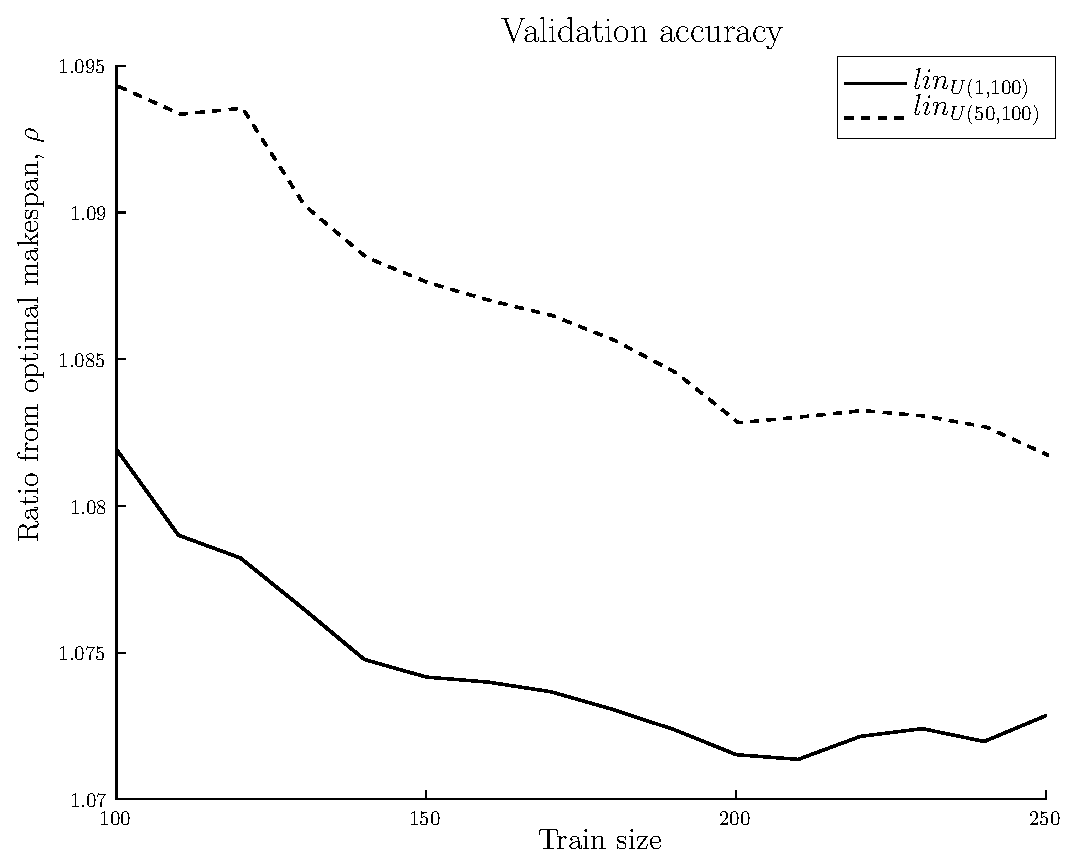
\includegraphics[width=5cm]{figs/fig1_trainsize.eps}
\caption{Deviation from optimal makespan as a function of size of training set. Solid line represents model $lin_{U(1,100)}$ and dashed line represents model $lin_{U(50,100)}$.}\end{figure}\end{center}
}
\frame{\frametitle{Training accuracy}
\begin{center}\begin{figure}[H] 
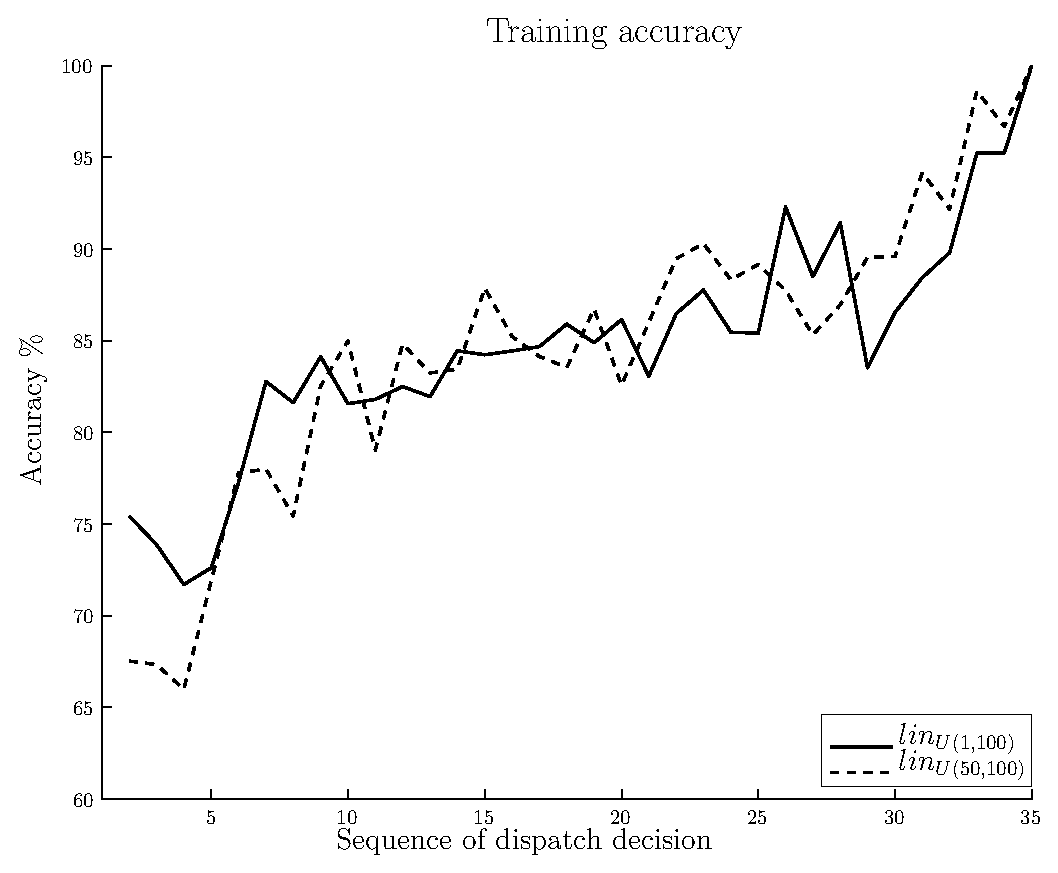
\includegraphics[width=5cm]{figs/fig2_trainacc.eps}
\caption{Training accuracy as a function of time. Solid line represents model $lin_{U(1,100)}$ and dashed line represents data distributions $lin_{U(50,100)}$}
\end{figure}\end{center}
}
\subsection{Main conclusions}
\frame{\frametitle{Comparing different dispatching rules}
\begin{figure}[t!]
\centering
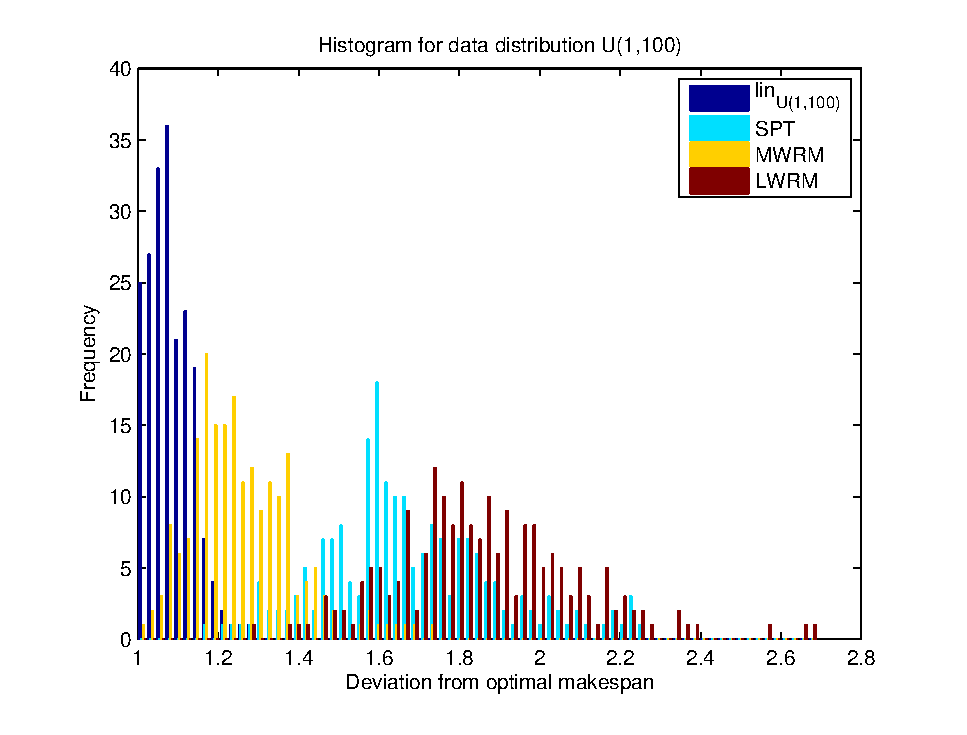
\includegraphics[width=4cm]{figs/fig3_hist_0_100_col.eps}
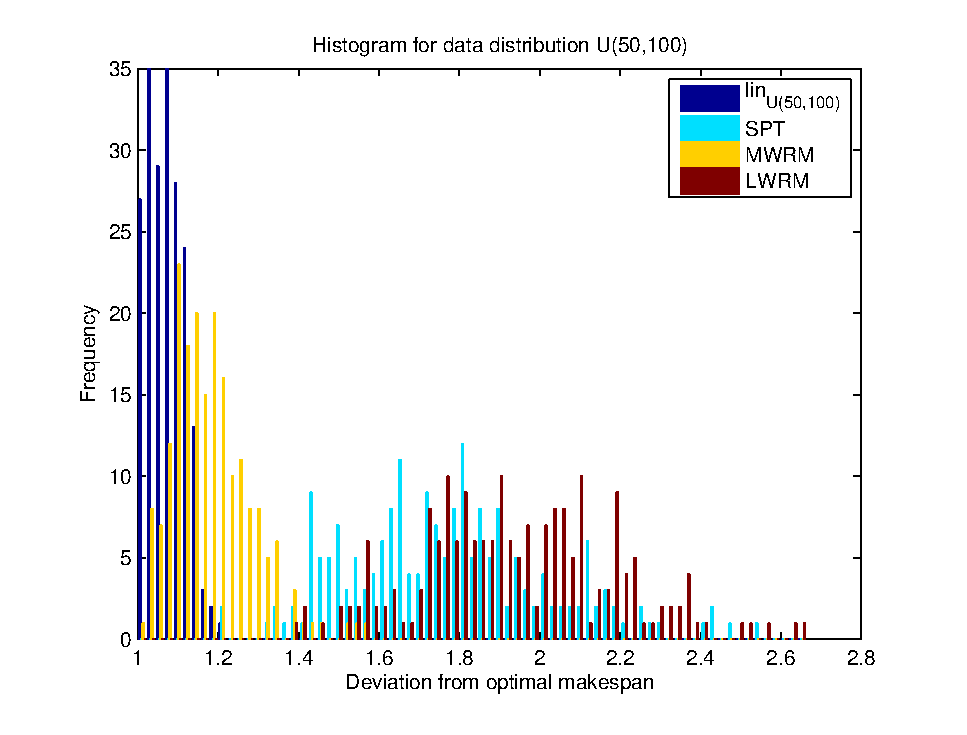
\includegraphics[width=4cm]{figs/fig3_hist_50_100_col.eps}
\caption{Histogram of deviation from optimal makespan for the dispatching rules $(lin_{U(R,100)})$, $(SPT)$, $(MWRM)$ and $(LWRM$). The figure on the left depicts model $lin_{U(1,100)}$, and the figure on the right is of model $lin_{U(50,100)}$.}
\label{fig:densities}
\end{figure}
}
\frame{\frametitle{Comparing different dispatching rules using ratio from optimality}
\begin{table}[t!]
 {\footnotesize
 \begin{center}
  \begin{tabular}{|p{1.5cm}|ccccc|}
   \hline\hline
   $U(1,100)$ & mean& std    & med    & min    & max   \\ \hline
   $lin_{U(1,100)}$ & 1.0842 & 0.0536 & 1.0785 & 1.0000 & 1.2722\\
   $SPT$     & 1.6707 & 0.2160 & 1.6365 & 1.1654 & 2.2500\\
   $MWRM$    & 1.2595 & 0.1307 & 1.2350 & 1.0000 & 1.7288\\
   $LWRM$    & 1.8589 & 0.2292 & 1.8368 & 1.2907 & 2.6906\\  
   \hline\hline
  \end{tabular}
  \begin{tabular}{|p{1.5cm}|ccccc|}
   \hline\hline
   $U(50,100)$ & mean   & std    & med    & min    & max    \\ \hline
   $lin_{U(50,100)}$    & 1.0724 & 0.0446 & 1.0713 & 1.0000 & 1.2159 \\
   $SPT$         & 1.7689 & 0.2514 & 1.7526 & 1.2047 & 2.5367 \\ 
   $MWRM$        & 1.1835 & 0.0994 & 1.1699 & 1.0217 & 1.5561 \\
   $LWRM$        & 1.9422 & 0.2465 & 1.9210 & 1.3916 & 2.6642 \\ 
   \hline\hline
  \end{tabular}
 \end{center}}
 \caption{Mean value, standard deviation, median value, minimum and maximum values using the test sets corresponding to data distributions $U(1,100)$ (above) and $U(50,100)$ (below) .}
 \label{tbl:stats}
\end{table}
}
\frame{\frametitle{Robustness towards data distribution using ratio from optimality}
\begin{table}[h!]
 {\footnotesize
 \begin{center}
  \begin{tabular}{|c|l|l|ccccc|}
   \hline\hline
   & model & test set & mean & std    & med    & min    & max   \\ \hline
\#1 & $lin_{U(1,100)}$ & $U(1,100)$ & 1.0844 & 0.0535 & 1.0786 & 1.0000 & 1.2722  \\
\#2 & $lin_{U(50,100)}$ & $U(1,100)$ & 1.0709 & 0.0497&1.0626 & 1.0000 & 1.2503  \\
\#3 & $lin_{U(1,100)}$ & $U(50,100)$ & 1.1429 & 0.1115&1.1158 & 1.0000 & 1.5963  \\
\#4 & $lin_{U(50,100)}$ & $U(50,100)$ & 1.0724 & 0.0446&1.0713 & 1.0000 & 1.2159  \\
%#4 and #1 are the same distribution
%#4 and #3 are the same distribution
   \hline\hline
  \end{tabular}
 \end{center}}
 \caption{Mean value, standard deviation, median value, minimum and maximum values for the test sets corresponding to data distributions $U(1,100)$ and $U(50,100)$, on both models $lin_{U(1,100)}$ and $lin_{U(50,100)}$.}
 \label{tbl:diffdatadistr}
\end{table}
}
\frame{\frametitle{Feature selection}
\begin{table}[h!]
 {\footnotesize
 \begin{center}
  \begin{tabular}{|c|r|r|p{5cm}|}
   \hline\hline
  weight & $lin_{U(1,100)}$ & $lin_{U(50,100)}$ & description \\ \hline
  $\bar{w}(1)$ &  -0.6712 & -0.2220 & processing time for job on machine\\
  $\bar{w}(2)$ &  -0.9785 & -0.9195 & work remaining \\
  $\bar{w}(3)$ & -1.0549  & -0.9059 & start-time \\
  $\bar{w}(4)$ & -0.7128  & -0.6274 & end-time \\
  $\bar{w}(5)$ & -0.3268  &  0.0103 & when machine is next free \\
  $\bar{w}(6)$ &  1.8678  &  1.3710 & current makespan \\
  $\bar{w}(7)$ & -1.5607  & -1.6290 & slack time for this particular machine \\
  $\bar{w}(8)$ & -0.7511  & -0.7607 & slack time for all machines \\
  $\bar{w}(9)$ & -0.2664  & -0.3639 & slack time weighted w.r.t. number of operations already assigned \\
   \hline\hline
  \end{tabular}
 \end{center}}
 \caption{Mean value, standard deviation, median value, minimum and maximum values for the test sets corresponding to data distributions $U(1,100)$ and $U(50,100)$, on both models $lin_{U(1,100)}$ and $lin_{U(50,100)}$.}
 \label{tbl:features}
\end{table}
}
\frame{\frametitle{Fixed weights vs. varied weights}
\begin{figure}[b!]
\centering
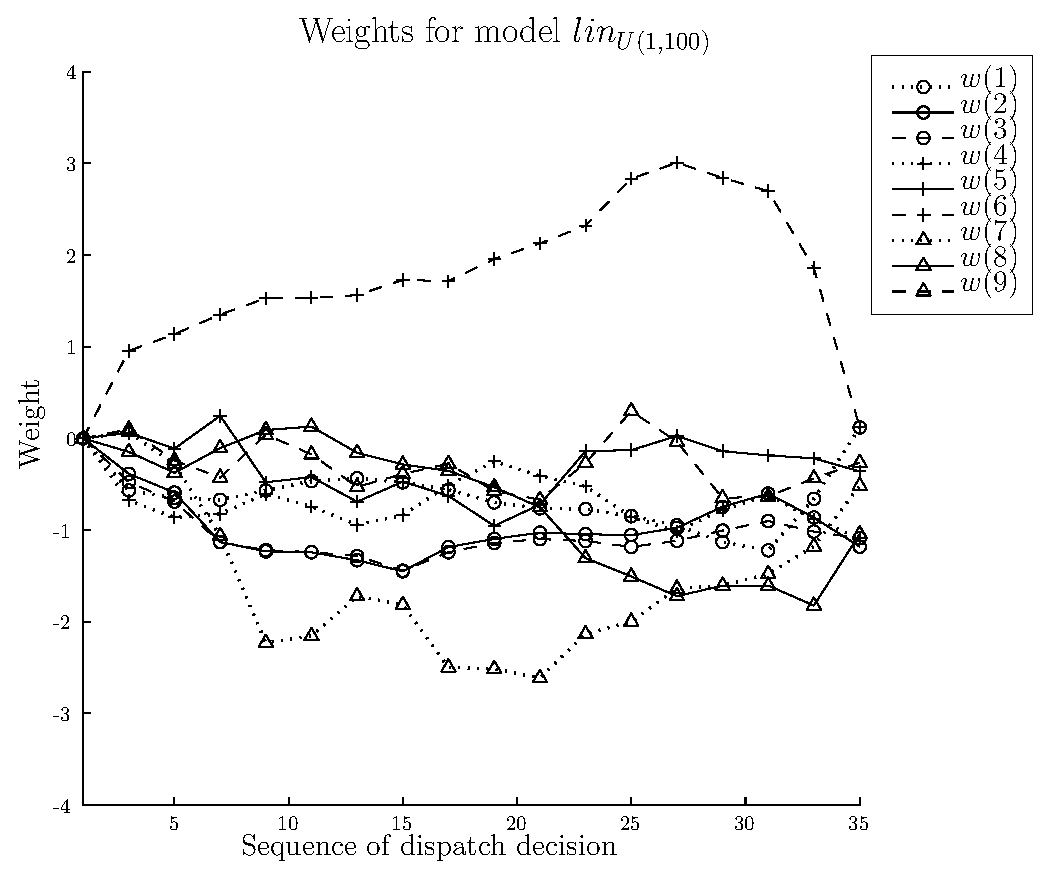
\includegraphics[width=0.45\columnwidth]{figs/fig6_weights0_100.eps}
\includegraphics[width=0.45\columnwidth]{figs/fig6_weights50_100.eps}
\caption{Weights of features as a function of time, for data distribution $U(1,100)$ (left) and $U(50,100)$ (right).}
\label{fig:variedweights}
\end{figure}
}
\frame{\frametitle{Robustness towards data distribution using fixed weights using ratio from optimality}
\begin{table}[h!]
 {\footnotesize
 \begin{center}
  \begin{tabular}{|c|l|l|ccccc|}
   \hline\hline
   & model & test set & mean & std    & med    & min    & max   \\ \hline
\#1 & $\bar{lin}_{U(1,100)}$ & $U(1,100)$ & 1.0862 & 0.0580 & 1.0785 & 1.0000 & 1.2722   \\
\#2 & $\bar{lin}_{U(50,100)}$ & $U(1,100)$ & 1.0706 & 0.0493 & 1.0597 & 1.0000 & 1.2204  \\
\#3 & $\bar{lin}_{U(1,100)}$ & $U(50,100)$ &   1.1356 & 0.0791 & 1.1296 & 1.0000 & 1.5284  \\
\#4 & $\bar{lin}_{U(50,100)}$ & $U(50,100)$ &  1.0695 & 0.0459 & 1.0658 & 1.0000 & 1.2201  \\
%#4 and #3 are the same distribution
   \hline\hline
  \end{tabular}
 \end{center}}
 \caption{Mean value, standard deviation, median value, minimum and maximum values for the test sets corresponding to data distributions $U(1,100)$ and $U(50,100)$, on both fixed weight models $\bar{lin}_{U(1,100)}$ and $\bar{lin}_{U(50,100)}$.}
 \label{tbl:diffdatadistr:fixed}
\end{table}
}

\section{Future Work}
{\frame{\frametitle{Future work}
\bi Overcome problems due to non unique sequence representation of JSSP
  \item Other learning methods, 
    \bi supervised learning, e.g. decision trees; 
    \item unsupervised learning, e.g. reinforcement learning;
   \ei
  \item Other data distributions and dimensions of JSSP
  \item Adding due dates to JSSP
\ei
}
\end{document}
%%%%%%%%%%%%%%%%%%%%%%%%%%%%%%%%%%%%%%%
